\chapter{Results}
\label{sec:results}
\section{Training Results}
%TODO: Add training results?

\section{Experiment Results}
\paragraph{}
\subsection{Results of experiments 1 and 2}
\paragraph{} Results for experiments 1 and 2 are shown respectively in the first two columns of Table~\ref{tab:results-input-features} and \ref{tab:results-other-features}. The third column indicates the group according to the description made in section \ref{sec:experiment-2}. The set of features is divided in input and non-input features, with reference to the input of the conditional network.
	
	\subsubsection{Input Features}
	\begin{longtable}{llll}
		\caption[Test results for input features]{ \small KS-test results for input features, using a significance level of 0.05 and the Bonferroni correction method. Results are indicated with R if the null hypothesis can be rejected or with N otherwise. An asterisk indicates the network that performed better (has the minimum KS distance) if the null hypothesis is rejected in every network}\\
		\toprule
		{} & uncond & cond & Group \\
		feature                   &        &      &       \\
		\midrule
		\endhead
		\midrule
		\multicolumn{3}{r}{{Continued on next page}} \\
		\midrule
		\endfoot
		
		\bottomrule
		\endlastfoot
		level\_equivalent\_diameter &      N &    N &    F3 \\
		level\_major\_axis\_length   &     R* &    R &    F1 \\
		level\_minor\_axis\_length   &      N &    N &    F3 \\
		level\_solidity            &      R &   R* &    F1 \\
		nodes                     &      R &   R* &    F1 \\
		distmap-skew              &      R &   R* &    F1 \\
		distmap-kurt              &      R &    N &    F2 \\
		\label{tab:results-input-features}
	\end{longtable}
	
	
	\subsubsection{Non-Input Features}	
	
	\begin{longtable}{llll}
		\caption[Test results for non input features]{ \small KS-test results for non-input features, using a significance level of 0.05 and the Bonferroni correction method. Results are indicated with R if the null hypothesis can be rejected or with N otherwise. An asterisk indicates the network that performed better (has the minimum KS distance) if the null hypothesis is rejected in every network}\\
		\toprule
		{} & uncond & cond & Group \\
		feature                       &        &      &       \\
		\midrule
		\endhead
		\midrule
		\multicolumn{3}{r}{{Continued on next page}} \\
		\midrule
		\endfoot
		
		\bottomrule
		\endlastfoot
		level\_area                    &      N &    N &    F3 \\
		level\_convex\_area             &      N &    N &    F3 \\
		level\_eccentricity            &     R* &    R &    F1 \\
		level\_euler\_number            &      R &   R* &    F1 \\
		level\_extent                  &      R &   R* &    F1 \\
		level\_filled\_area             &      N &    N &    F3 \\
		level\_orientation             &      N &    N &    F3 \\
		level\_perimeter               &      N &    N &    F3 \\
		level\_hu\_moment\_0             &      N &    R &    F4 \\
		level\_hu\_moment\_1             &     R* &    R &    F1 \\
		level\_hu\_moment\_2             &      R &   R* &    F1 \\
		level\_hu\_moment\_3             &      R &    N &    F2 \\
		level\_hu\_moment\_4             &      N &    R &    F4 \\
		level\_hu\_moment\_5             &      N &    R &    F4 \\
		level\_hu\_moment\_6             &      R &    N &    F2 \\
		level\_centroid\_x              &     R* &    R &    F1 \\
		level\_centroid\_y              &     R* &    R &    F1 \\
		number\_of\_artifacts           &      R &   R* &    F1 \\
		number\_of\_powerups            &      R &    N &    F2 \\
		number\_of\_weapons             &      R &   R* &    F1 \\
		number\_of\_ammunitions         &     R* &    R &    F1 \\
		number\_of\_keys                &      R &   R* &    F1 \\
		number\_of\_monsters            &     R* &    R &    F1 \\
		number\_of\_obstacles           &      R &   R* &    F1 \\
		number\_of\_decorations         &      R &   R* &    F1 \\
		walkable\_area                 &      N &    N &    F3 \\
		walkable\_percentage           &      N &    N &    F3 \\
		start\_location\_x\_px           &      R &   R* &    F1 \\
		start\_location\_y\_px           &      R &   R* &    F1 \\
		artifacts\_per\_walkable\_area   &      R &   R* &    F1 \\
		powerups\_per\_walkable\_area    &      R &    N &    F2 \\
		weapons\_per\_walkable\_area     &      R &   R* &    F1 \\
		ammunitions\_per\_walkable\_area &     R* &    R &    F1 \\
		keys\_per\_walkable\_area        &      R &   R* &    F1 \\
		monsters\_per\_walkable\_area    &      R &   R* &    F1 \\
		obstacles\_per\_walkable\_area   &      R &   R* &    F1 \\
		decorations\_per\_walkable\_area &      R &   R* &    F1 \\
		avg-path-length               &      R &   R* &    F1 \\
		diameter-mean                 &      R &   R* &    F1 \\
		art-points                    &     R* &    R &    F1 \\
		assortativity-mean            &     R* &    R &    F1 \\
		betw-cen-min                  &      N &    N &    F3 \\
		betw-cen-max                  &      R &   R* &    F1 \\
		betw-cen-mean                 &     R* &    R &    F1 \\
		betw-cen-var                  &     R* &    R &    F1 \\
		betw-cen-skew                 &      R &   R* &    F1 \\
		betw-cen-kurt                 &      R &   R* &    F1 \\
		betw-cen-Q1                   &     R* &    R &    F1 \\
		betw-cen-Q2                   &     R* &    R &    F1 \\
		betw-cen-Q3                   &     R* &    R &    F1 \\
		closn-cen-min                 &     R* &    R &    F1 \\
		closn-cen-max                 &      R &   R* &    F1 \\
		closn-cen-mean                &     R* &    R &    F1 \\
		closn-cen-var                 &      R &   R* &    F1 \\
		closn-cen-skew                &     R* &    R &    F1 \\
		closn-cen-kurt                &     R* &    R &    F1 \\
		closn-cen-Q1                  &     R* &    R &    F1 \\
		closn-cen-Q2                  &      R &   R* &    F1 \\
		closn-cen-Q3                  &      R &   R* &    F1 \\
		distmap-max                   &     R* &    R &    F1 \\
		distmap-mean                  &     R* &    R &    F1 \\
		distmap-var                   &     R* &    R &    F1 \\
		distmap-Q1                    &     R* &    R &    F1 \\
		distmap-Q2                    &      R &   R* &    F1 \\
		distmap-Q3                    &      R &   R* &    F1 \\
		\label{tab:results-other-features}
	\end{longtable}
\subsection{Graphical results for Experiments 1 and 2}
%TODO: Go on from here
\begin{figure}[ht] 
	\label{fig:results-input-feats} 
	\begin{minipage}[b]{0.5\linewidth}
		\centering
		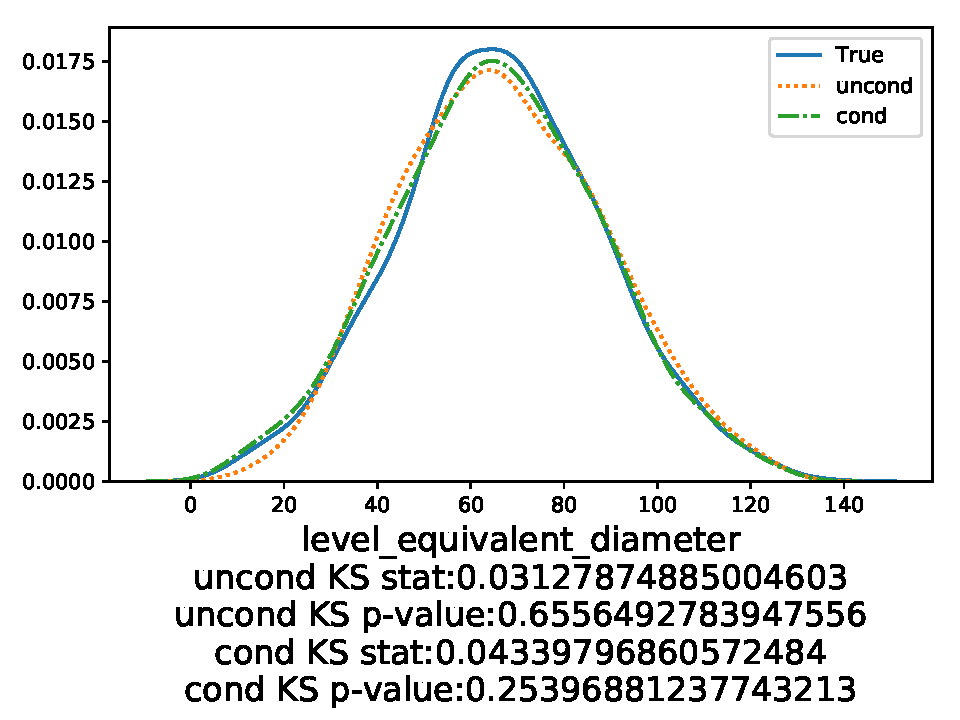
\includegraphics[width=\linewidth]{results/exp1-2/level_equivalent_diameter.pdf} 
		\caption[Results: Experiments 1 and 2, level\_equivalent\_diameter]{Results: Experiments 1 and 2, level\_equivalent\_diameter.} 
		\vspace{4ex}
	\end{minipage}%%
	\begin{minipage}[b]{0.5\linewidth}
		\centering
		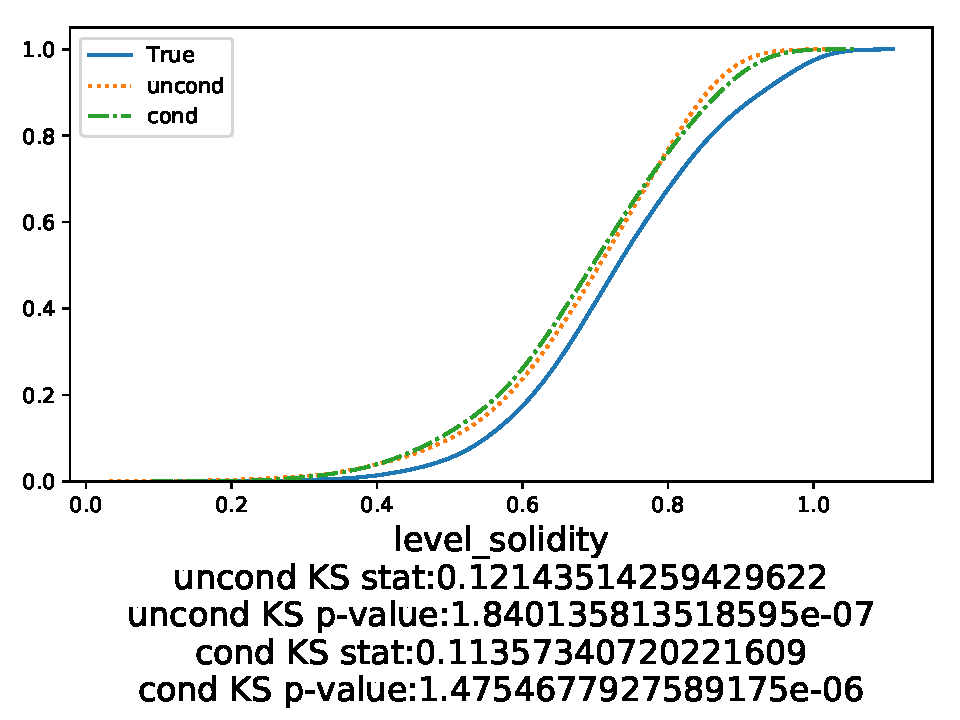
\includegraphics[width=\linewidth]{results/exp1-2/level_solidity.pdf} 
		\caption[Results: Experiments 1 and 2, level\_equivalent\_diameter]{Results: Experiments 1 and 2, level\_equivalent\_diameter.} 
		\vspace{4ex}
	\end{minipage} 
\end{figure}

\begin{figure}[ht] 
	\begin{minipage}[b]{0.5\linewidth}
		\centering
		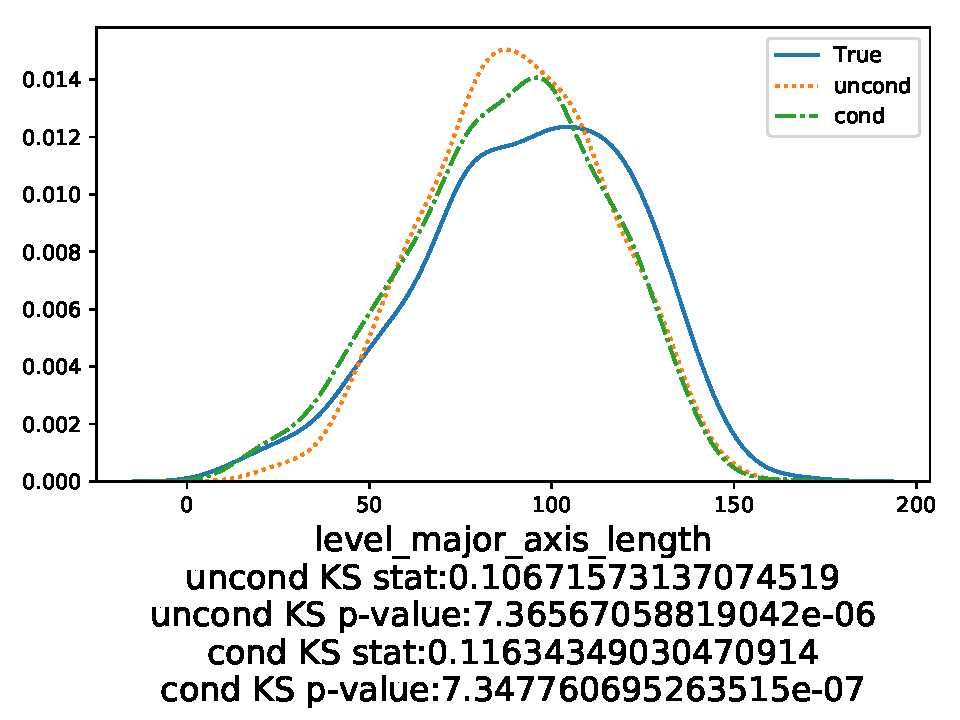
\includegraphics[width=\linewidth]{results/exp1-2/level_major_axis_length.pdf} 
		\caption{DFT, Initial condition} 
		\vspace{4ex}
	\end{minipage}
	\begin{minipage}[b]{0.5\linewidth}
		\centering
		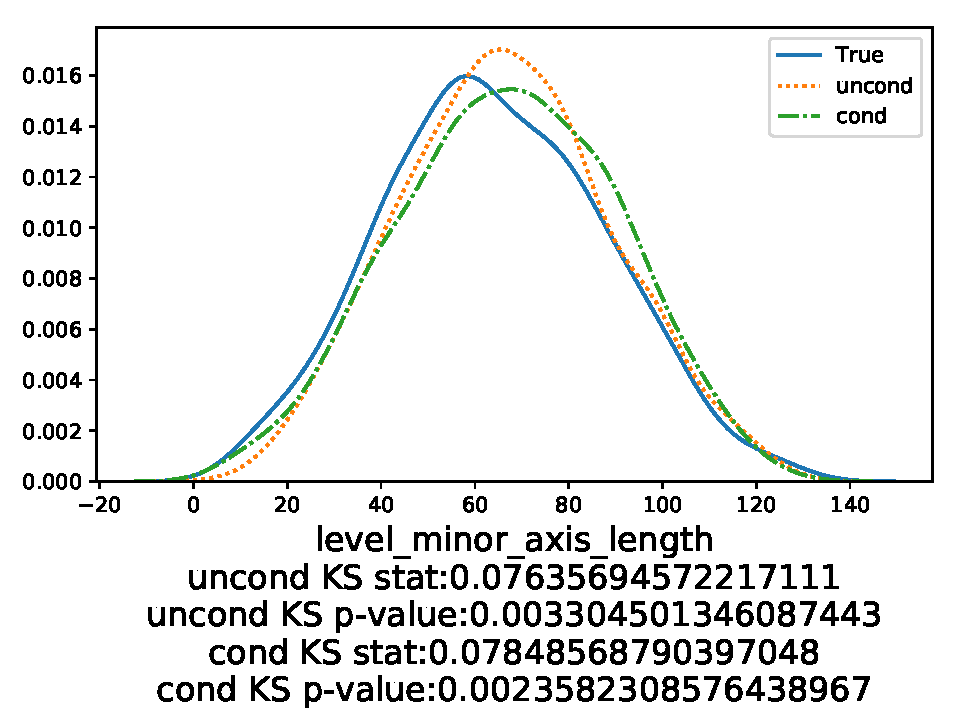
\includegraphics[width=\linewidth]{results/exp1-2/level_minor_axis_length.pdf} 
		\caption{DFT, rupture} 
		\vspace{4ex}
	\end{minipage} 
\end{figure}

\begin{figure}[ht] 
	\begin{minipage}[b]{0.5\linewidth}
		\centering
		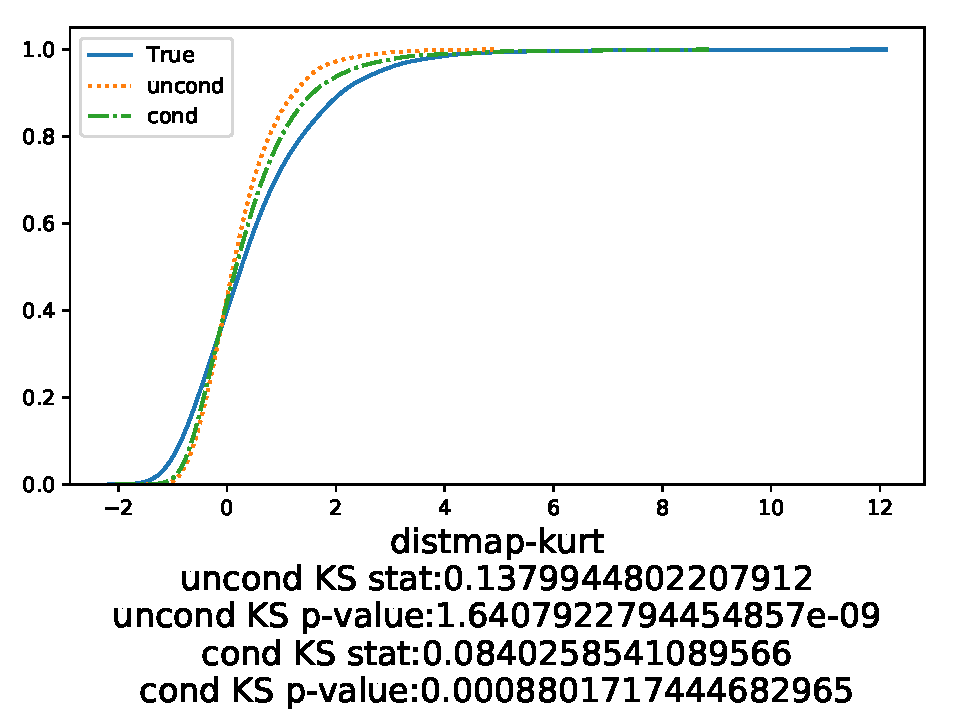
\includegraphics[width=\linewidth]{results/exp1-2/distmap-kurt.pdf} 
		\caption{DFT, rupture} 
		\vspace{4ex}
	\end{minipage} 
	\begin{minipage}[b]{0.5\linewidth}
	\centering
	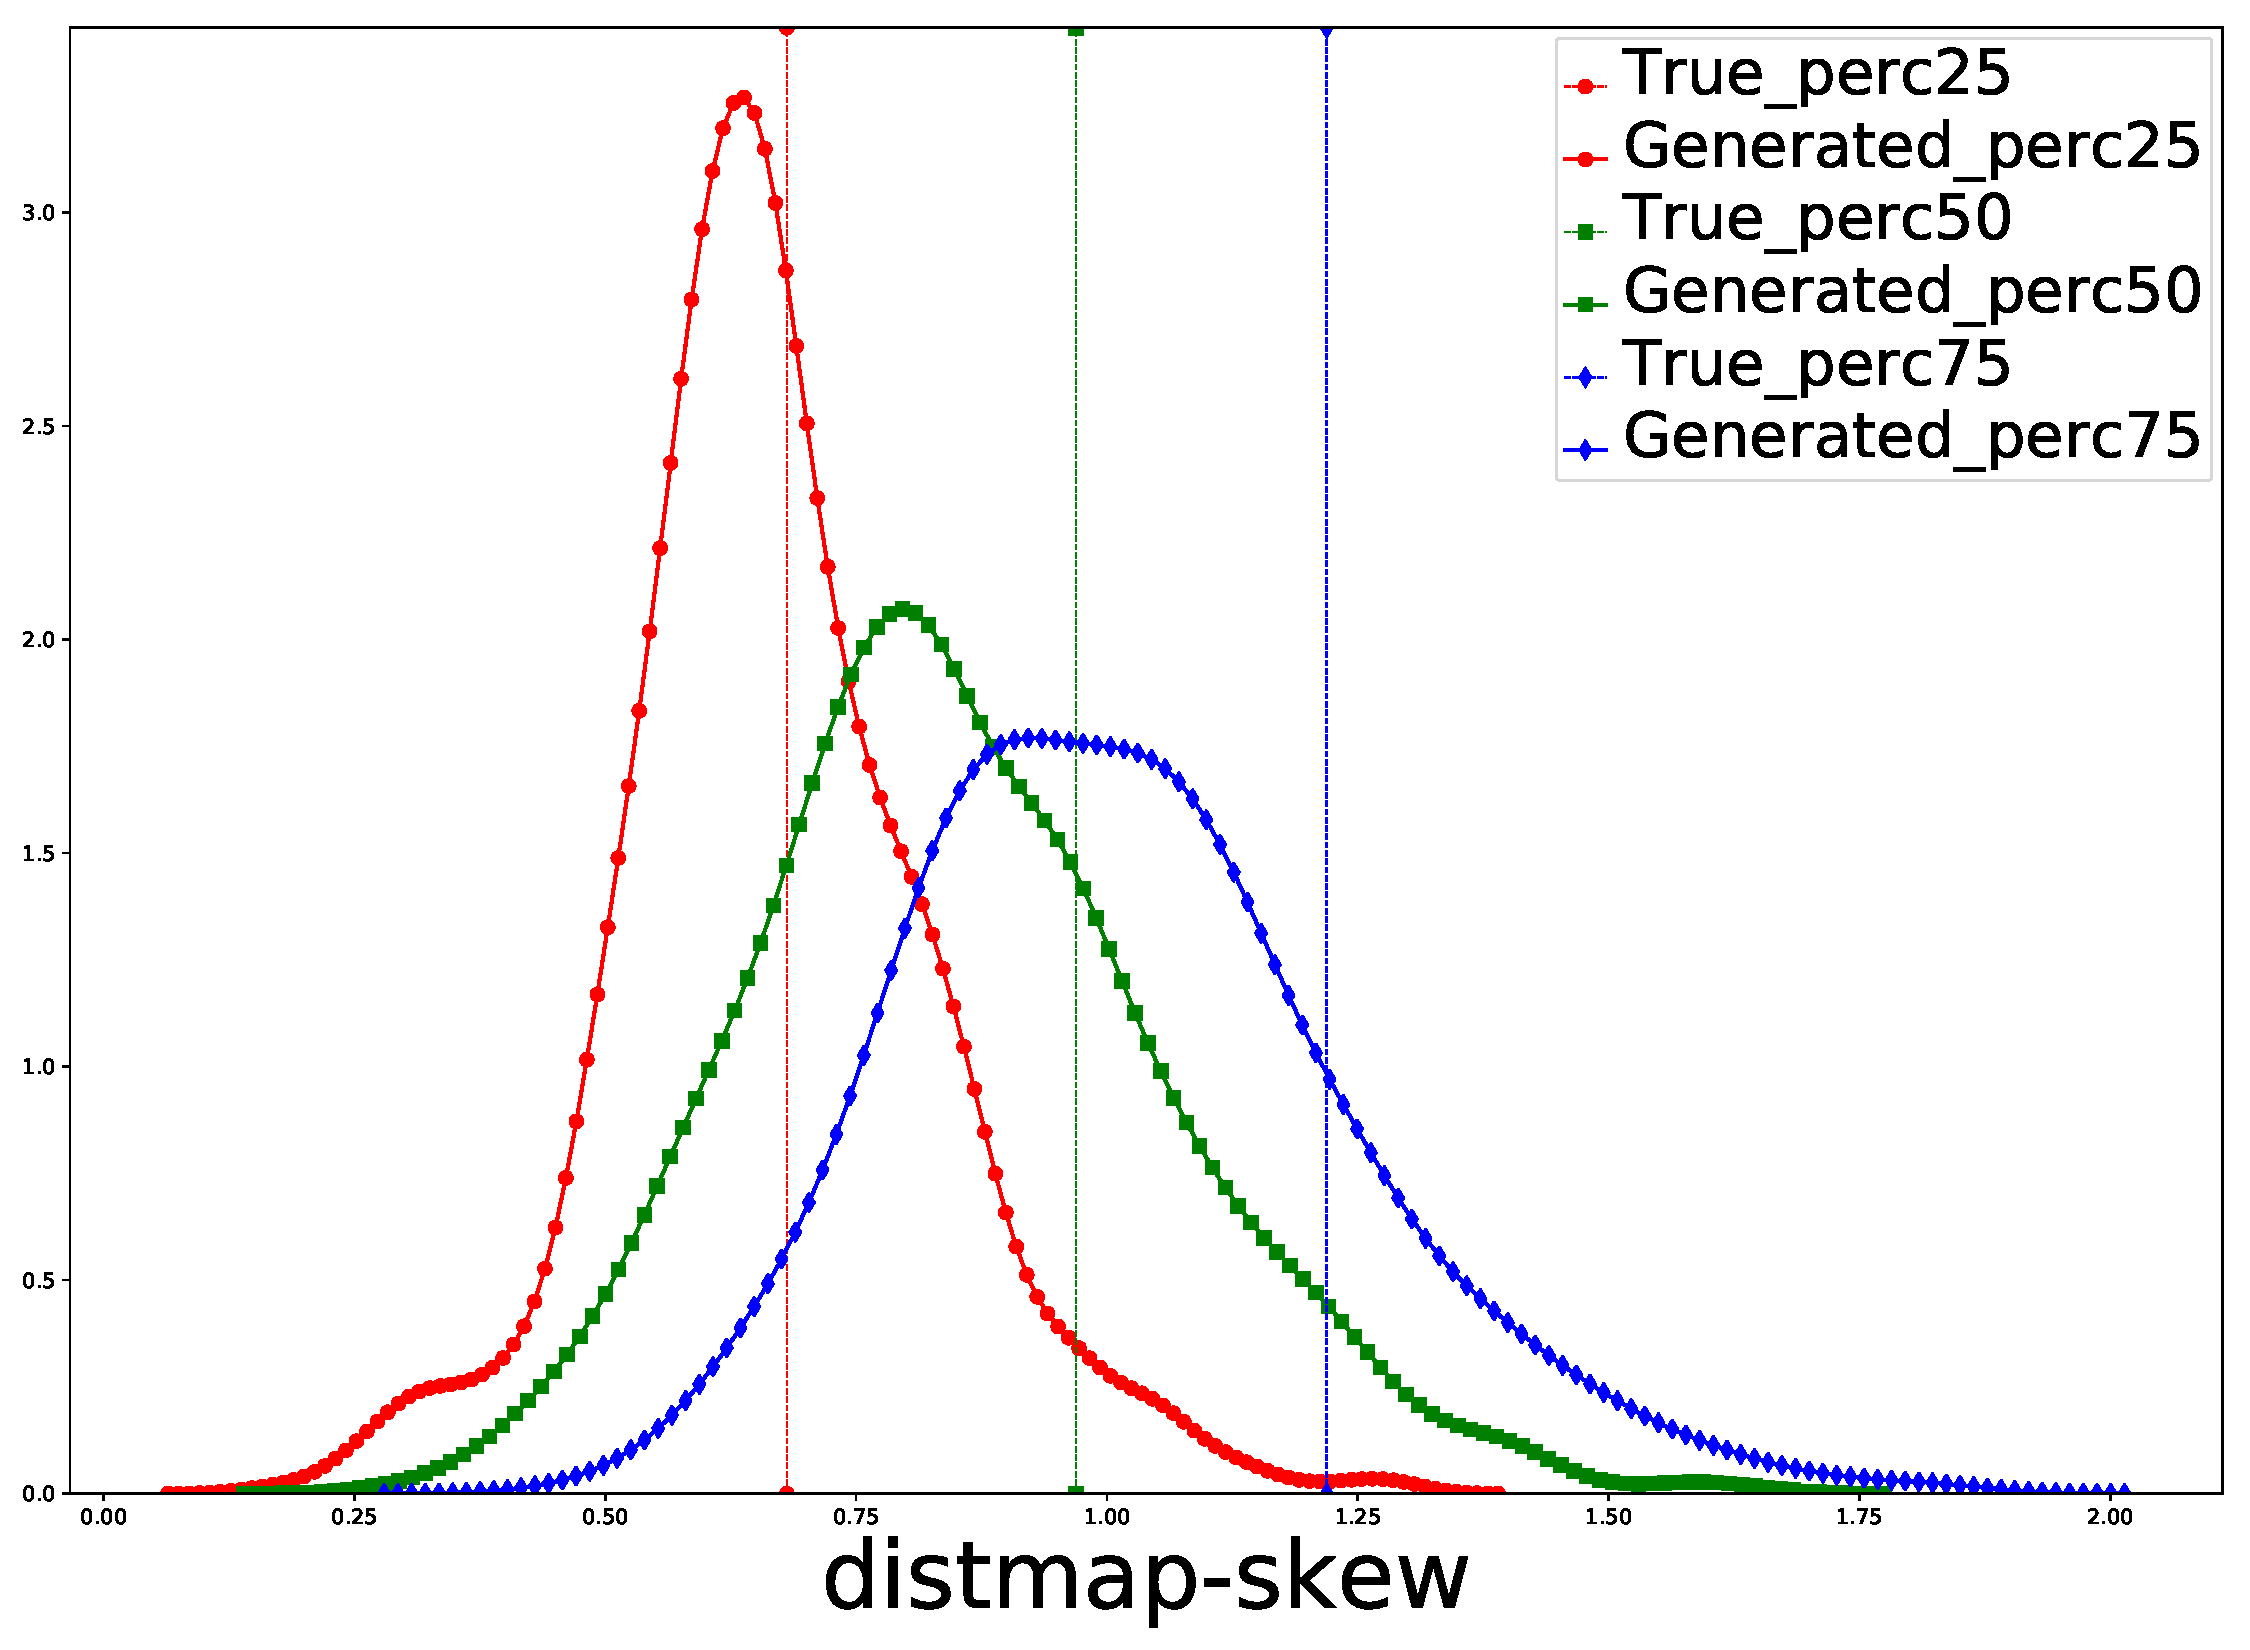
\includegraphics[width=\linewidth]{results/exp1-2/distmap-skew.pdf} 
	\caption{DFT, rupture} 
	\vspace{4ex}
	\end{minipage} 
\end{figure}

\begin{figure}[ht] 
	\centering
		\begin{minipage}[b]{0.5\linewidth}
		\centering
		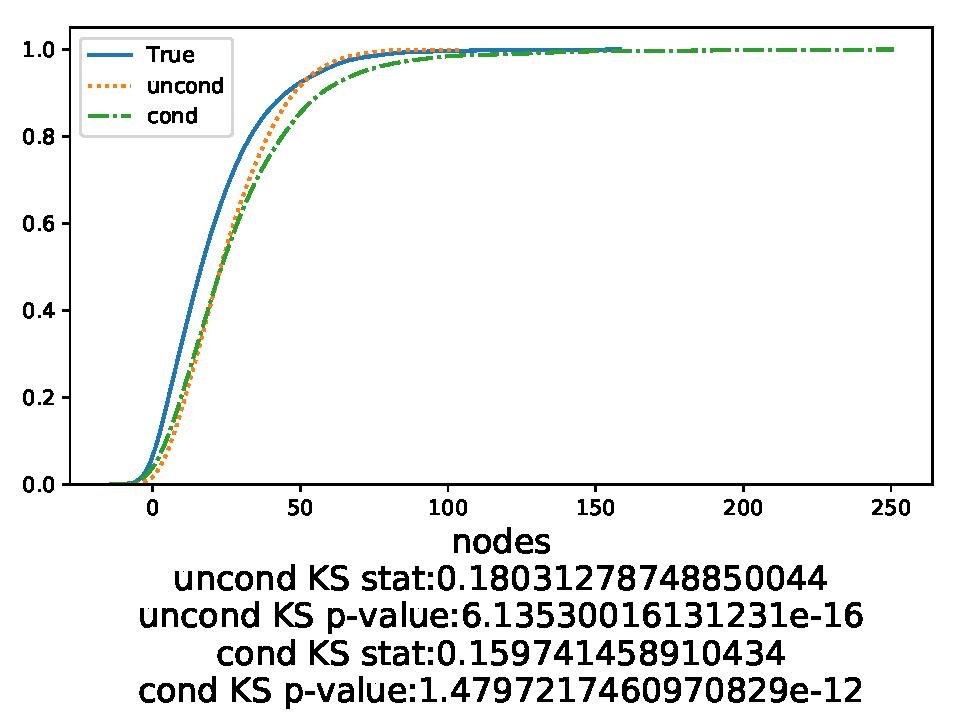
\includegraphics[width=\linewidth]{results/exp1-2/nodes.pdf} 
		\caption{DFT, rupture} 
		\vspace{4ex}
	\end{minipage} 
\end{figure}
\subsection{Results of Experiment 3}



\section{Generated Samples}
\section{Summary}